\apendice{Documentación de usuario}

\section{Introducción}
En esta sección, se explica al usuario qué necesita para poder utilizar la aplicación, cómo se instalaría y un manual de usuario para enseñarle cómo funciona.

\section{Requisitos de usuarios} \label{requisitos}
Los requisitos necesarios para poder utilizar la aplicación web son:

\begin{itemize}
	\item Tener un navegador que soporte HTML5, como Google Chrome o Microsoft Edge.
	\item Tener conexión a Internet.
\end{itemize}

Además, dado que es necesario estar dado de alta para utilizar la aplicación, se han preparado unos usuarios específicos para poder realizar pruebas en la aplicación desde un usuario con privilegios y otro sin privilegios:

\begin{itemize}
	\item \underline{Administrador:} 
	\begin{itemize}
		\item \textbf{Nombre de usuario:} admin.
		\item \textbf{Contraseña:} 1234.
	\end{itemize}
	\item \underline{Usuario:}
	\begin{itemize}
		\item \textbf{Nombre de usuario:} usuario.
		\item \textbf{Contraseña:} 1234.
	\end{itemize}
\end{itemize}

También en la \textit{release} del repositorio de \href{https://github.com/xam1002/TFG_Deteccion_Parkinson}{GitHub} hay un archivo \textit{.pkl} con el que se puede modificar el modelo.

\section{Instalación}
Al tratarse de una aplicación web, no necesita nada más allá de un navegador web que soporte HTML5. Únicamente sería suficiente con acceder a aplicación web mediante el \href{http://tfg.identificacionparkinson.es:5000/}{enlace}.

\section{Manual del usuario}
En esta sección se explica cómo utilizar la aplicación web.

\subsection{Inicio de sesión}
Nada más acceder a la aplicación web, aparecerá la pantalla de inicio de sesión que representa la figura \ref{fig:inicio_sesion_E}. Para acceder a ella, es necesario estar previamente dado de alta. Los usuarios indicados en el punto \ref{requisitos} pueden ser utilizados para acceder a la aplicación.

En caso de no escribir correctamente el usuario, aparecerá un mensaje indicando que el usuario es incorrecto, como se aprecia en la figura \ref{fig:usuario_no_encontrado_E}. Si la contraseña es incorrecta, aparecerá otro mensaje indicando que el error en el inicio de sesión ha sido la contraseña, tal y como se muestra en la figura \ref{fig:clave_incorrecta_E}, pero teniendo en cuenta que el usuario es correcto.

Dependiendo de si se trata de un usuario con o sin privilegios, aparecerán unas opciones u otras.

\begin{figure}[ht]
	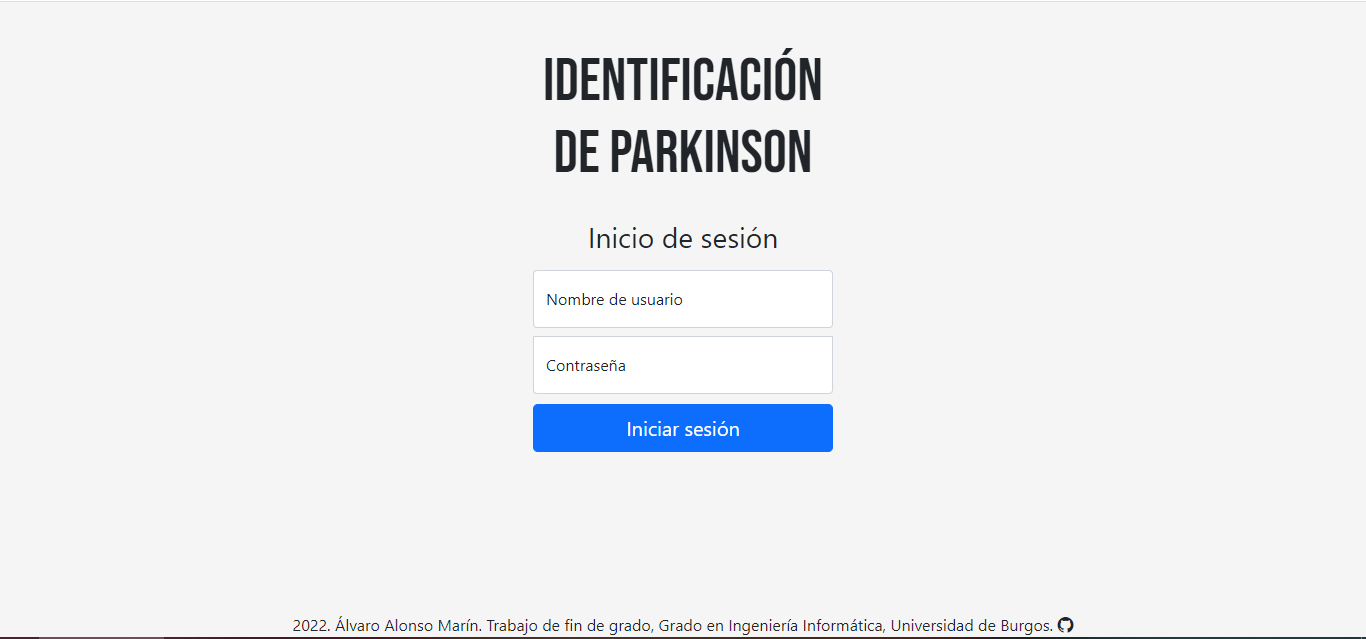
\includegraphics[width=1\textwidth]{inicio_sesion_E}
	\caption{Pantalla del inicio sesión de la aplicación web.}
	\label{fig:inicio_sesion_E}
\end{figure}

\begin{figure}[ht]
	\includegraphics[width=1\textwidth]{usuario_no_encontrado_E}
	\caption{Pantalla del inicio sesión con el error de usuario no encontrado.}
	\label{fig:usuario_no_encontrado_E}
\end{figure}

\begin{figure}[ht]
	\includegraphics[width=1\textwidth]{clave_incorrecta_E}
	\caption{Pantalla del inicio sesión con el error de contraseña inválida.}
	\label{fig:clave_incorrecta_E}
\end{figure}

\subsection{Pantalla principal}

\subsubsection{Usuario administrador}
En caso de haber accedido con el usuario administrador, se podrán realizar más operaciones. En esta pantalla se podrá seleccionar el vídeo o arrastrarlo para realizar la predicción, además de seleccionar la mano y el sexo, tal y como se muestra en la figura \ref{fig:pantalla_principal_admin_E}.

\begin{figure}[ht]
	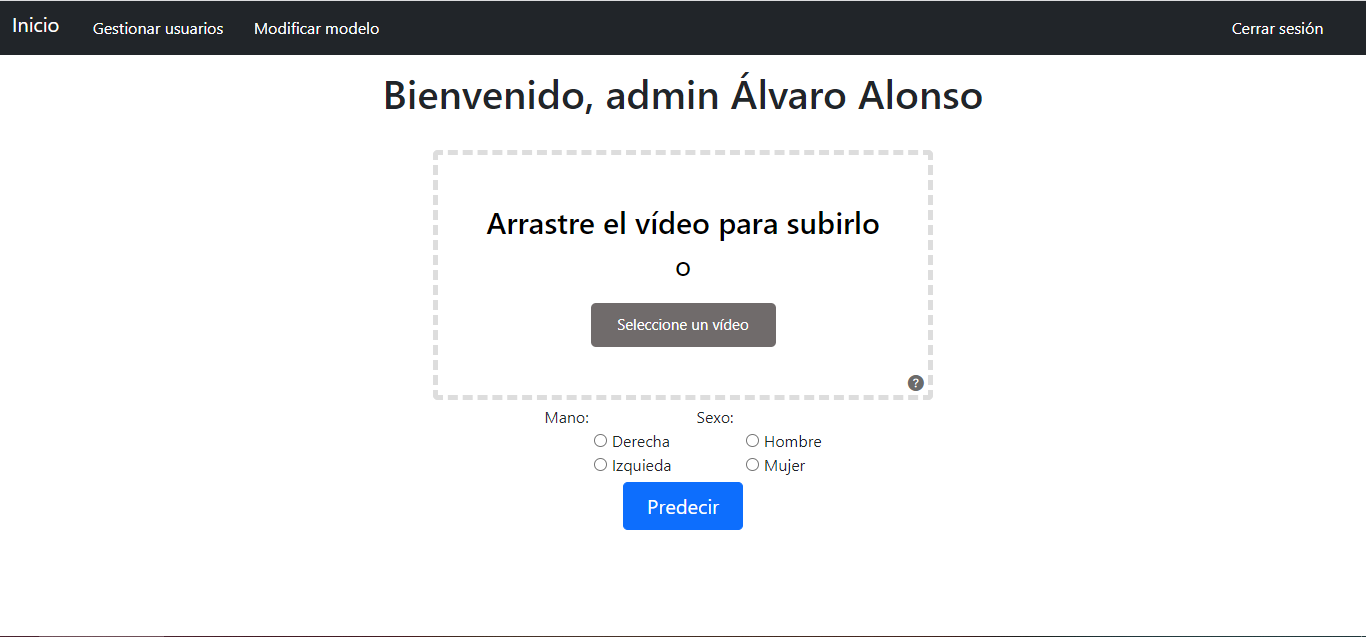
\includegraphics[width=1\textwidth]{pantalla_principal_admin_E}
	\caption{Pantalla principal del administrador para realizar la predicción.}
	\label{fig:pantalla_principal_admin_E}
\end{figure}

Además, es necesario rellenar todos los campos, ya que si no no se podrá realizar la predicción y se mostrarán mensajes de error. Estos mensajes pueden aparecer cuando no se rellenen los campos, como se puede ver en la figura \ref{fig:se_deben_rellenar_campos_E}, mientras que si el formato del archivo no es correcto aparecerá el mensaje que se aprecia en la figura \ref{fig:archivo_no_valido_E}.

\begin{figure}[ht]
	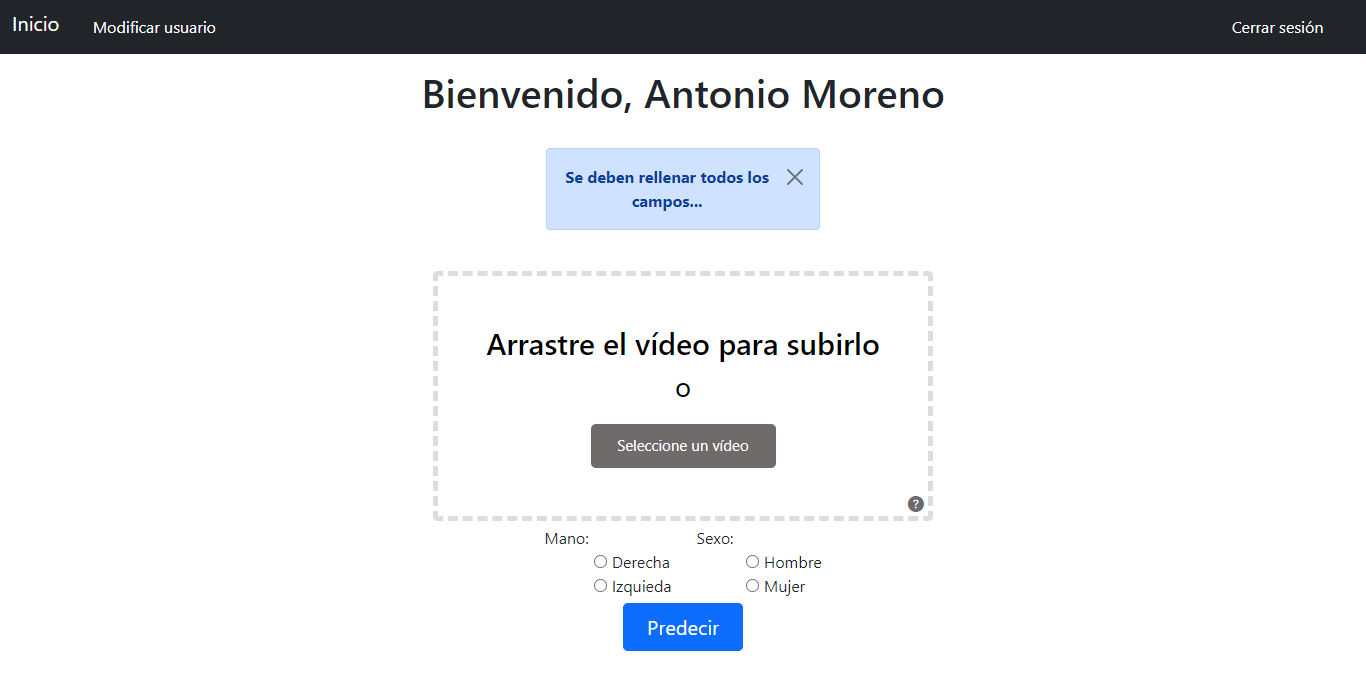
\includegraphics[width=1\textwidth]{se_deben_rellenar_campos_E}
	\caption{Pantalla principal del administrador con el mensaje de que se deben rellenar todos los campos.}
	\label{fig:se_deben_rellenar_campos_E}
\end{figure}

\begin{figure}[ht]
	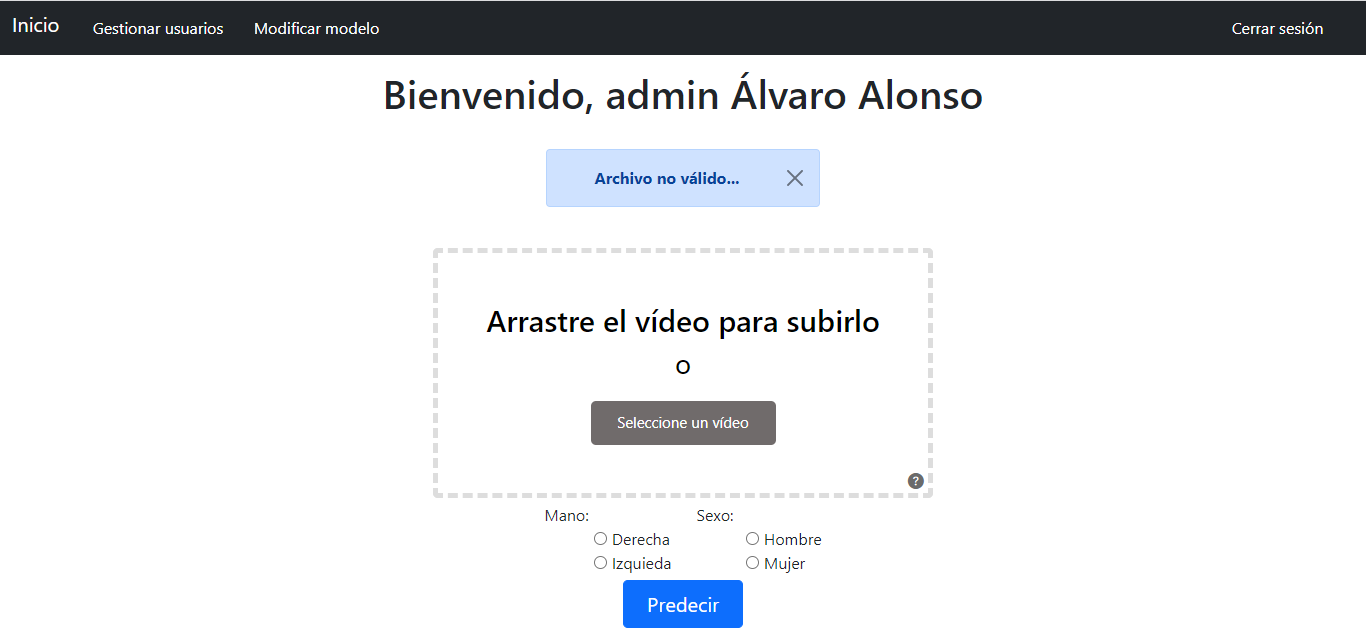
\includegraphics[width=1\textwidth]{archivo_no_valido_E}
	\caption{Pantalla principal del administrador con el mensaje de que el archivo no es válido.}
	\label{fig:archivo_no_valido_E}
\end{figure}

\subsubsection{Usuario sin privilegios}
La diferencia con el usuario administrador reside en las funcionalidades que a las que no tiene acceso un usuario sin privilegios.

La única diferencia es la barra de navegación, ya que el usuario sin privilegios no podrá ni gestionar usuarios ni modificar el modelo, aunque sí que podrá modificar su propia información de usuario, tal y como se muestra en la figura \ref{fig:pantalla_principal_E}.

\begin{figure}[ht]
	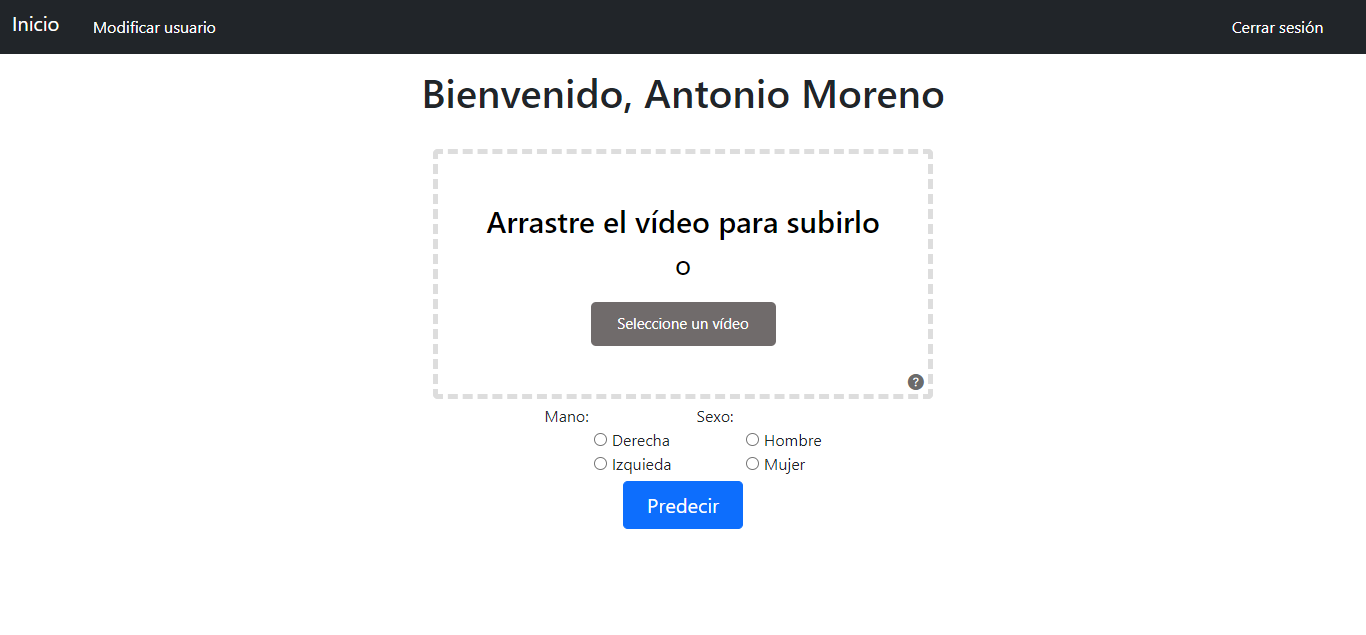
\includegraphics[width=1\textwidth]{pantalla_principal_E}
	\caption{Pantalla principal de un usuario sin privilegios para realizar la predicción.}
	\label{fig:pantalla_principal_E}
\end{figure}

\subsection{Realizar predicción}
Tras añadir un vídeo y seleccionar la mano y el sexo, aparecerá una pantalla\footnote{Dado que ya se ha explicado en el paso anterior la diferencia entre un usuario administrador y un usuario sin privilegios, se va a continuar el resto del punto E.4 mostrando capturas del administrador, teniendo en cuenta que la parte de la predicción es idéntica en un usuario y en otro.} indicando al usuario que debe esperar, como se puede apreciar en la figura \ref{fig:cargando_E}. Dado que el servidor necesita procesar cada fotograma del vídeo, este proceso puede tardar varios minutos, que dependerá de la duración del vídeo.

\begin{figure}[ht]
	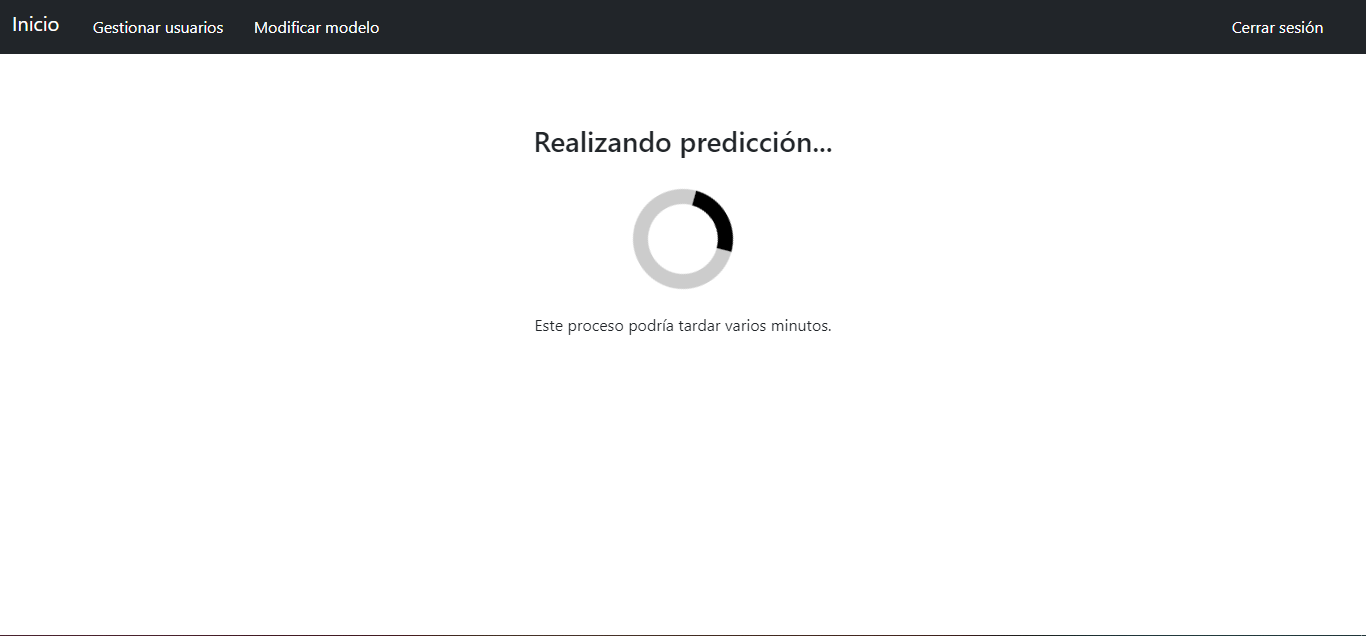
\includegraphics[width=1\textwidth]{cargando_E}
	\caption{Pantalla de carga mientras se realiza la predicción.}
	\label{fig:cargando_E}
\end{figure}

En caso de que no se pueda realizar la predicción, bien porque el vídeo sea erróneo o bien por otros motivos, aparecerá la pantalla que se puede ver en la figura \ref{fig:error_prediccion}.

\begin{figure}[ht]
	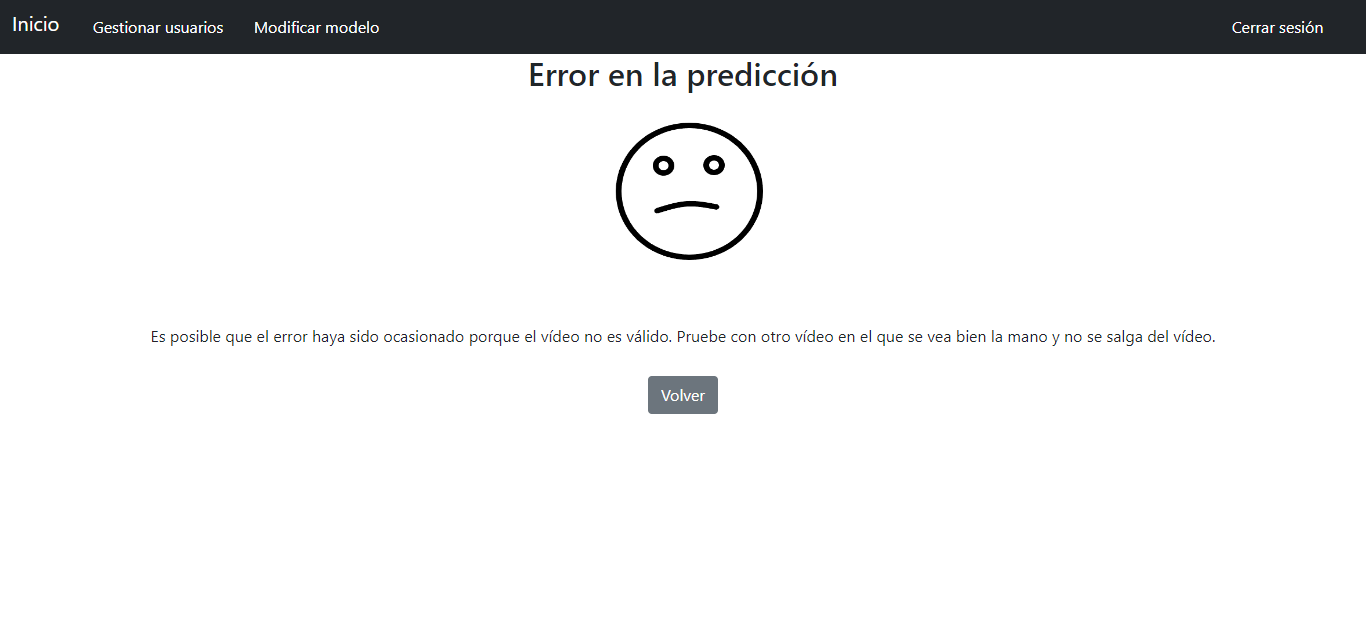
\includegraphics[width=1\textwidth]{error_prediccion}
	\caption{Pantalla que aparece cuando hay un error en la predicción.}
	\label{fig:error_prediccion}
\end{figure}

Una vez termine, aparecerá el resultado expresado en porcentaje, indicando cuál es la probabilidad de que la persona de la mano tenga Parkinson junto a si la probabilidad es baja (menos del 33 \%), media (entre el 33 \% y el 67 \%) y alta (más del 67 \%). Además, también hay un aviso sobre que la predicción ha sido realizada utilizando un \textit{software} de inteligencia artificial, por lo que para confirmar esta predicción habría que consultar con el médico. Todo esto se puede observar en la figura \ref{fig:resultado_E}.

\begin{figure}[ht]
	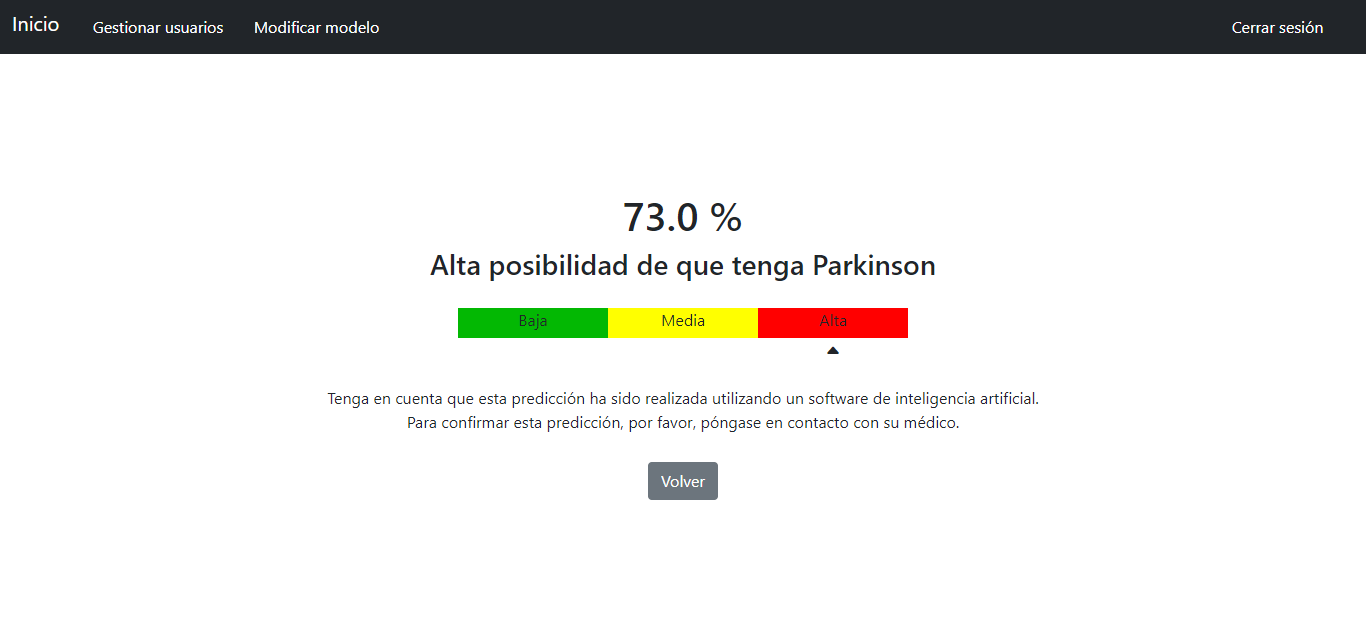
\includegraphics[width=1\textwidth]{resultado_E}
	\caption{Pantalla con el resultado de la predicción.}
	\label{fig:resultado_E}
\end{figure}

En la barra de navegación, se puede volver a la pantalla inicial haciendo clic en ``Inicio'' al igual que con el botón ``Volver'' en cualquier pantalla de la aplicación.

\subsection{Gestión de usuarios}
Como ya se ha explicado, el único usuario que puede acceder a esta pantalla es el administrador. Se puede acceder a ella mediante la opción ``Gestionar usuarios'' de la barra de navegación. Tras acceder, aparecerá la pantalla mostrada en la figura \ref{fig:gestion_usuarios_E}, en la que se listan todos los usuarios dados de alta en la aplicación junto a la posibilidad de modificar o eliminar cada uno de ellos. Además, se puede volver a la pantalla principal o añadir un nuevo usuario.

\begin{figure}[ht]
	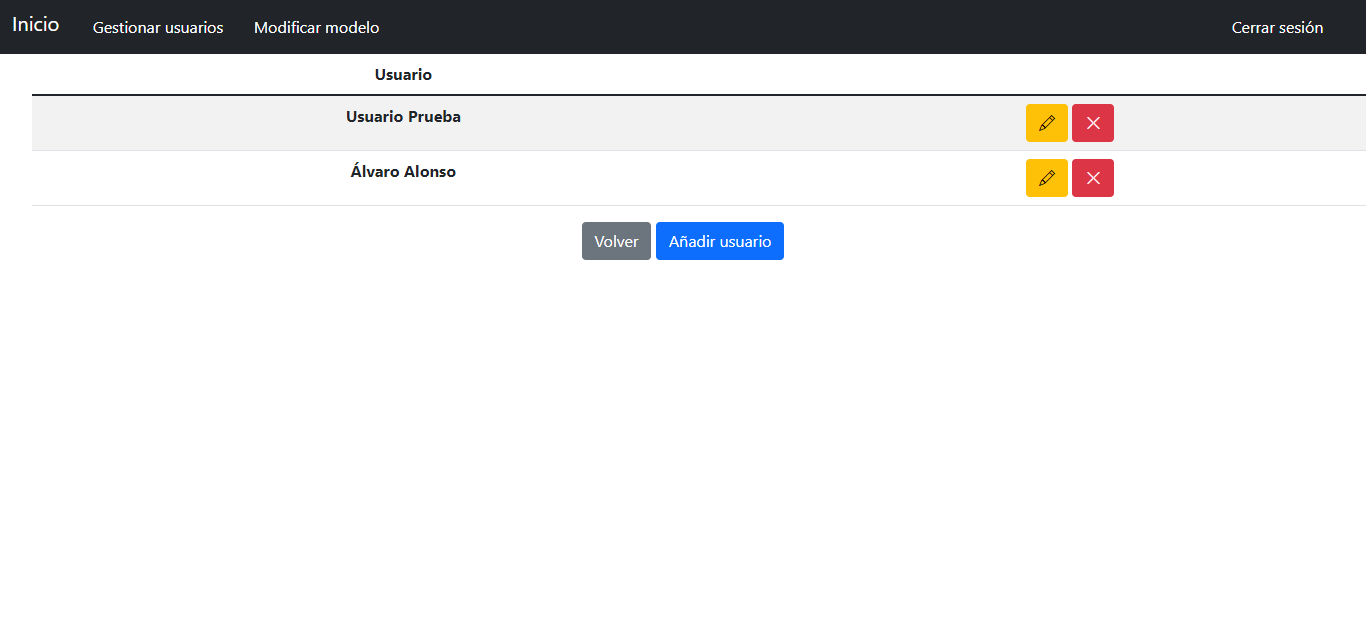
\includegraphics[width=1\textwidth]{gestion_usuarios_E}
	\caption{Pantalla de la gestión de usuarios.}
	\label{fig:gestion_usuarios_E}
\end{figure}

Cuando se selecciona la opción de ``Añadir usuario'', aparecerá un formulario donde habrá que rellenar los campos de nombre completo, nombre de usuario, contraseña y la repetición de la contraseña, tal y como se observa en la figura \ref{fig:agregar_usuario_E}

\begin{figure}[ht]
	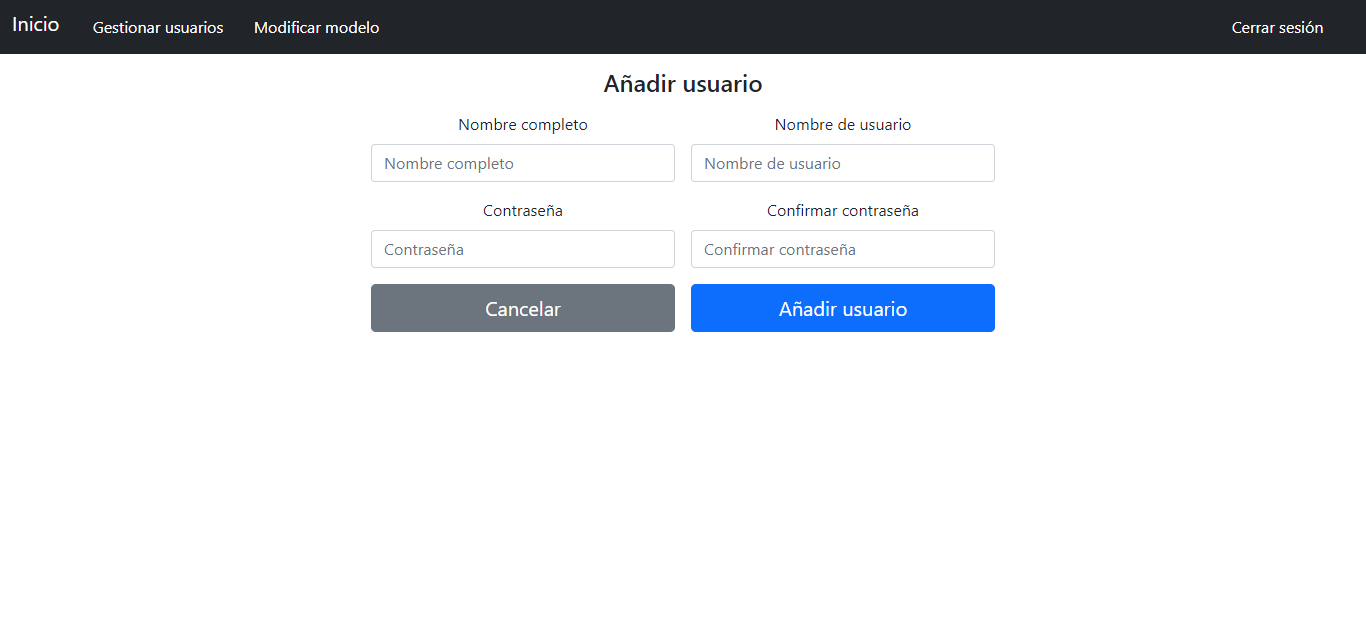
\includegraphics[width=1\textwidth]{agregar_usuario_E}
	\caption{Pantalla para añadir un usuario.}
	\label{fig:agregar_usuario_E}
\end{figure}

Es importante rellenar todos los campos, además de escribir un nombre de usuario que no exista y escribir la contraseña dos veces bien para que el usuario se dé de alta.

Cuando se selecciona el icono de modificar un usuario (\textit{i. e.} el botón amarillo con un lapicero), la pantalla que aparecerá será muy parecida a la anterior, como se puede ver en la figura \ref{fig:modificar_usuario_E}, pero con la diferencia de que vendrán los datos del usuarios ya escritos a excepción de la contraseña, para facilitar la modificación del usuario.

\begin{figure}[ht]
	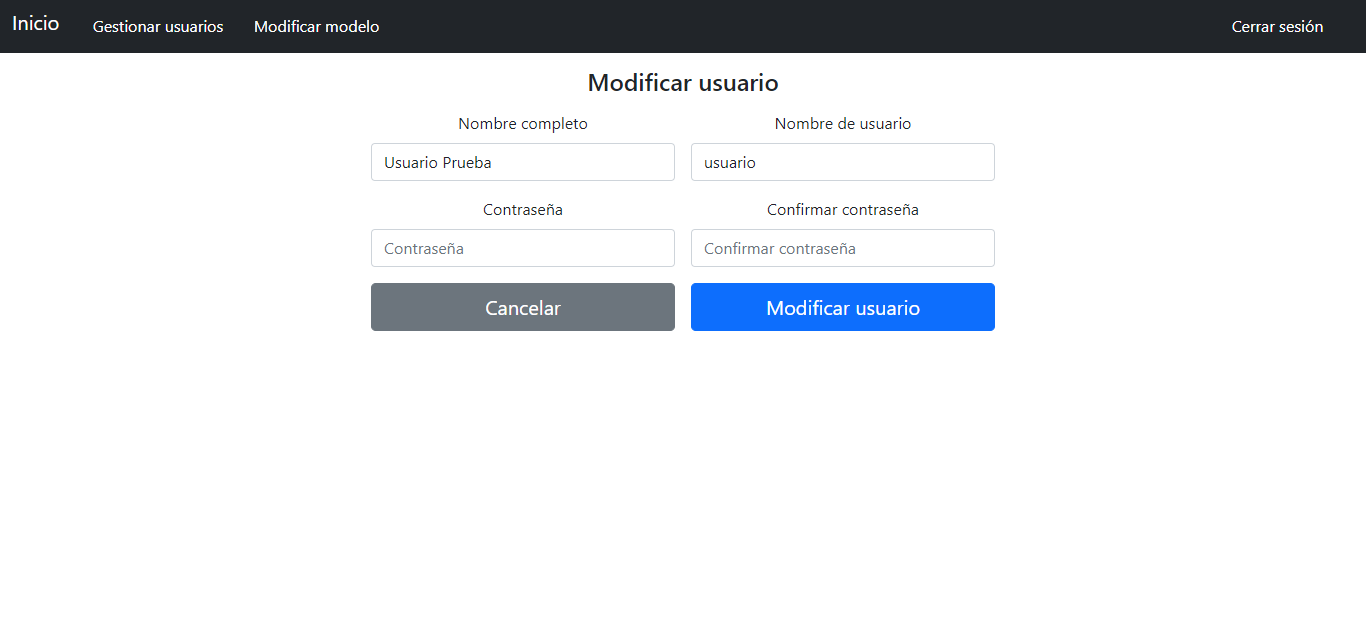
\includegraphics[width=1\textwidth]{modificar_usuario_E}
	\caption{Pantalla para modificar un usuario.}
	\label{fig:modificar_usuario_E}
\end{figure}

Un usuario sin privilegios podrá acceder a esta ventana únicamente para modificar su usuario, mediante la opción ``Modificar usuario'' de la barra de navegación.

Nuevamente, es importante que el nombre de usuario no exista, que todos los campos estén rellenos y que los campos de las contraseñas coincidan.

Cuando se selecciona el icono de modificar un usuario (\textit{i. e.} el botón rojo con una X), aparecerá una ventana emergente de confirmación, como se puede ver en la figura \ref{fig:eliminar_usuario_E}, con el objetivo de confirmar la operación o cancelarla.

\begin{figure}[ht]
	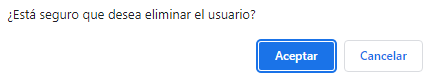
\includegraphics[width=0.8\textwidth]{eliminar_usuario_E}
	\caption{Mensaje de confirmación para eliminar un usuario.}
	\label{fig:eliminar_usuario_E}
\end{figure}

Tras realizar cualquiera de estas acciones se regresa a la pantalla de gestión de usuarios, salvo en el caso de que un usuario sin privilegios modifique su usuario, ya que volverá a la pantalla principal al no tener permiso para gestionar los usuarios.

\subsection{Modificar modelo}
Al igual que en la gestión de usuarios, esta pantalla sólo es accesible desde el administrador. Su funcionamiento es bastante parecido a la pantalla principal. Para actualizar el modelo, basta con arrastrar el modelo o seleccionarlo mediante el botón ``Seleccione un modelo''. Esta pantalla se puede apreciar en la figura \ref{fig:modificar_modelo_E}.

\begin{figure}[ht]
	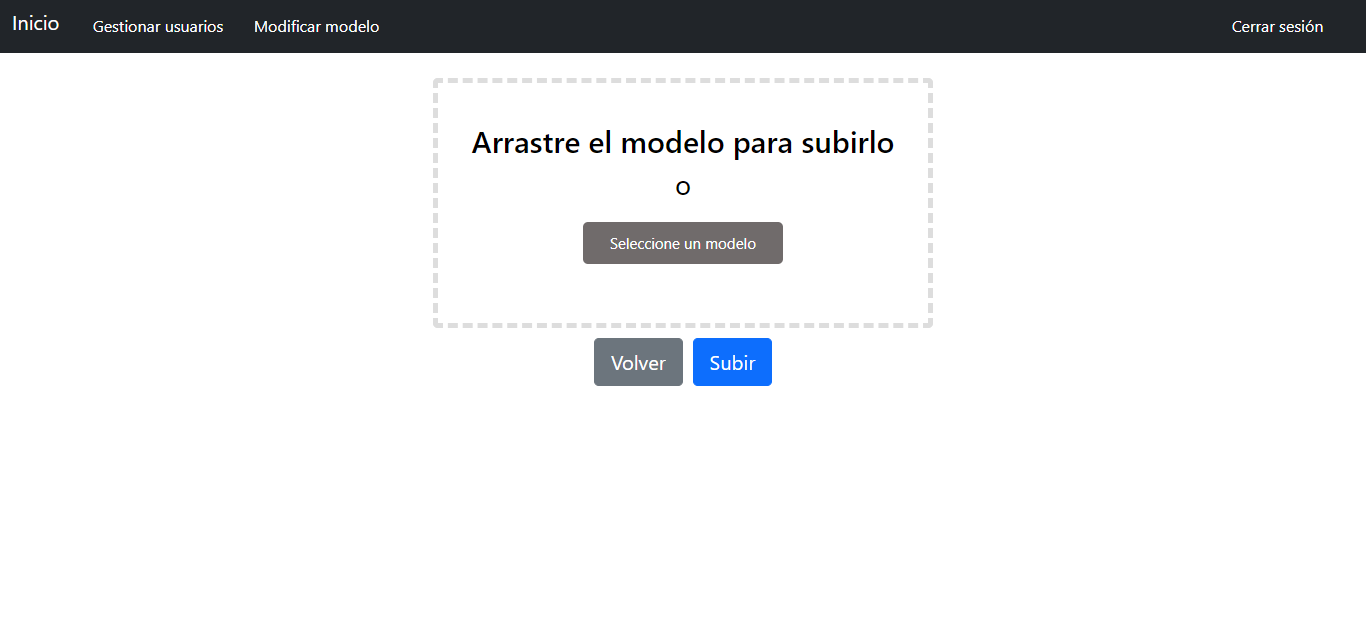
\includegraphics[width=1\textwidth]{modificar_modelo_E}
	\caption{Pantalla para modificar el modelo.}
	\label{fig:modificar_modelo_E}
\end{figure}

También aparecerá un error en caso de que el archivo que contiene el modelo no sea válido, como se puede observar en la figura \ref{fig:error_modelo_E}

\begin{figure}[ht]
	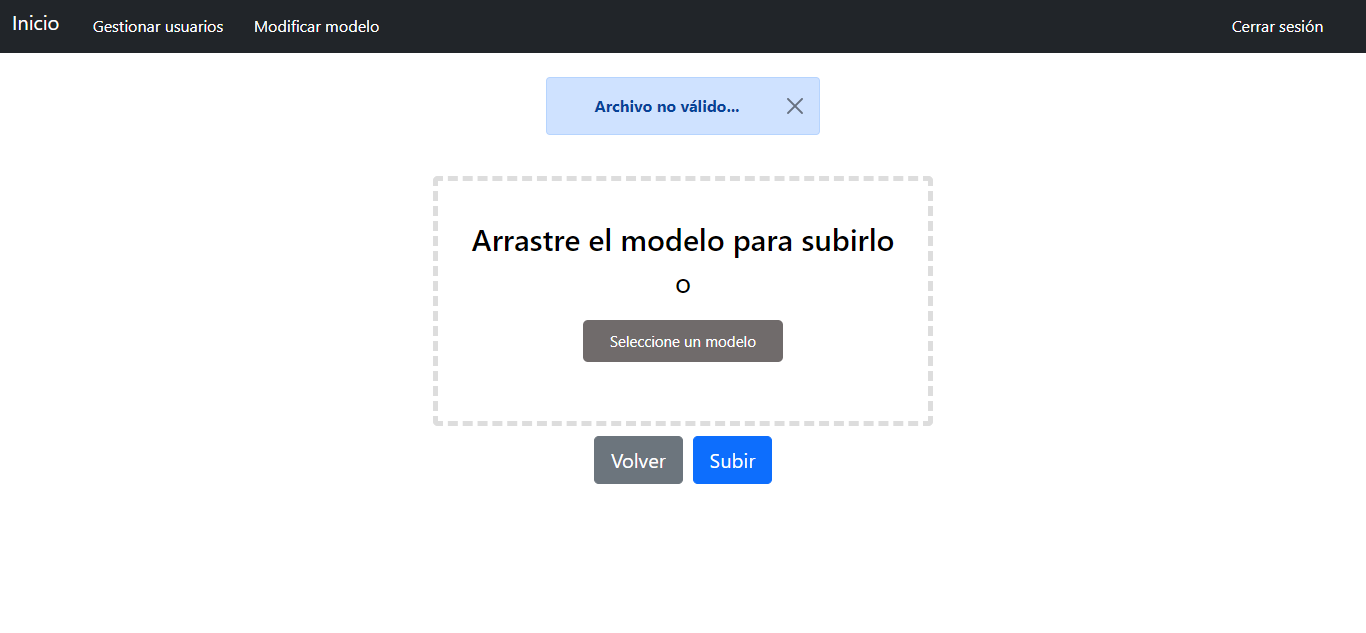
\includegraphics[width=1\textwidth]{error_modelo_E}
	\caption{Pantalla con un mensaje de error al modificar el modelo.}
	\label{fig:error_modelo_E}
\end{figure}

\subsection{Versión para pantallas pequeñas}
Cuando se acceda a la aplicación web con una pantalla pequeña, la barra de navegación cambiará ligeramente. Las opciones de la barra de navegación, pasarán a un menú desplegable accesible desde el icono de la izquierda y cambiará la opción de ``Cerrar sesión'' por un botón de apagado, tal y como se ve en las figuras \ref{fig:pantalla_principal_menu_desplegable_E} y \ref{fig:menu_desplegable_E}.

\begin{figure}[ht]
	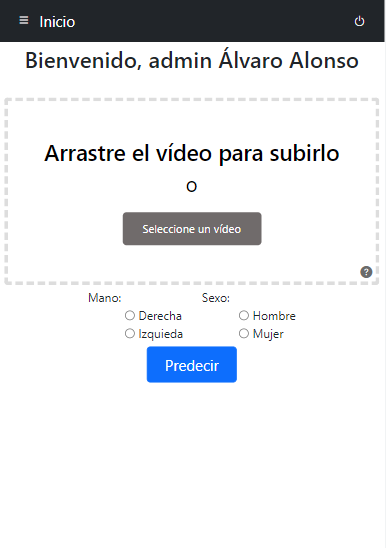
\includegraphics[width=0.8\textwidth]{pantalla_principal_menu_desplegable_E}
	\caption{Pantalla principal para pantallas pequeñas.}
	\label{fig:pantalla_principal_menu_desplegable_E}
\end{figure}

\begin{figure}[ht]
	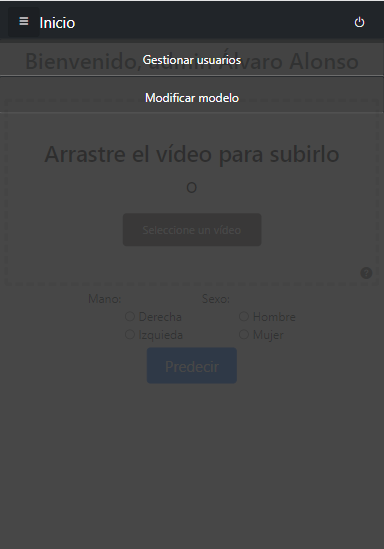
\includegraphics[width=0.8\textwidth]{menu_desplegable_E}
	\caption{Menú desplegable para pantallas pequeñas.}
	\label{fig:menu_desplegable_E}
\end{figure}
